\documentclass[10pt,a4paper]{article}
\usepackage[margin=1.7cm]{geometry}
\usepackage[T1]{fontenc}
\usepackage{lmodern}
\usepackage{graphicx}
\usepackage{enumitem}
\usepackage{xcolor}
\usepackage[hidelinks]{hyperref}
\usepackage{xurl}
\graphicspath{{figures/}}
\setlist{itemsep=3pt,topsep=3pt,leftmargin=12pt}
\pagestyle{empty}

\begin{document}

\begin{center}
{\Large\bfseries Synthetic 12-Lead ECG Generation for Imbalanced Rhythm Classification}\\[3pt]
{\large One-page summary}\\[3pt]
Shivank Mishra \quad$\cdot$\quad 2024ADPS0823G \quad$\cdot$\quad November 2026\\[2pt]
{\small Full report: \path{report/report.pdf} \quad Code and demo:
\url{https://github.com/shivankmishra144droid/Quality-Aware-Synthetic-Data-Augmentation-for-ECG-Classification}}
\end{center}

\noindent\textbf{Problem.} In PTB-XL's four rhythm classes (sinus rhythm, atrial fibrillation, sinus tachycardia,
sinus bradycardia), sinus rhythm makes up about 85\,\% of the data. Can generated ECGs help a rhythm classifier, does
choosing the \emph{best} synthetic ECGs help more than choosing random ones, and how realistic can a generator be?
Each study was pre-registered; the latent diffusion work uses only training and validation data.

\medskip
\noindent\fbox{\parbox{\dimexpr\linewidth-2\fboxsep-2\fboxrule}{
\textbf{Final generator: C-M.} Autoencoder (12$\times$1000 $\rightarrow$ 16$\times$125 latent) + S4 latent diffusion
model (5.9\,M parameters, 100k steps on Colab and Kaggle GPUs).\\[2pt]
\textbf{Realism on held-out validation patients} (feature-judge AUC; 0.5 = indistinguishable from real):
C-M \textbf{0.796} vs hand-built beat stitching 0.965 (pre-registered verdict: \textbf{better}).
Real-vs-real floor 0.454, autoencoder ceiling 0.627. No training ECG is copied.}}

\medskip
\begin{center}
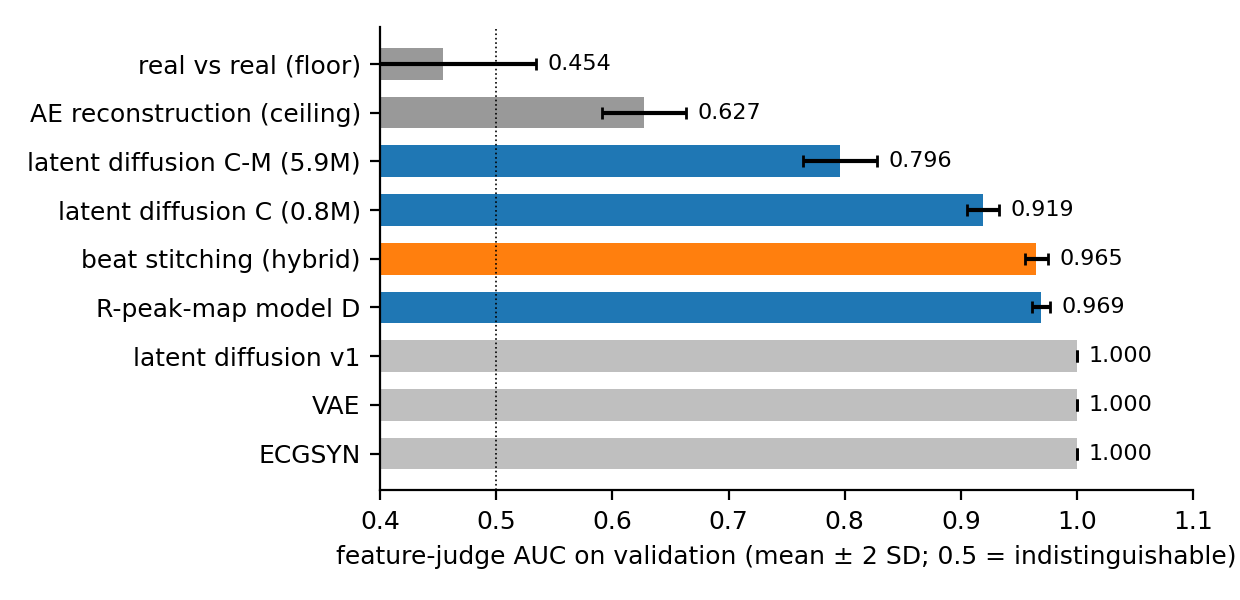
\includegraphics[width=0.62\linewidth]{fig_realism_ladder.png}
\end{center}

\noindent\textbf{Key findings}
\begin{itemize}
\item \textbf{Beat stitching works as a first generator.} Learned beat templates assembled by a rhythm model: a
  classifier trained only on these ECGs reaches 0.678 balanced accuracy on real ECGs (0.873 when trained on real ones).
\item \textbf{Quality filtering ranks samples but does not beat random selection.} Top-scored synthetic ECGs train a
  better classifier on their own (0.743 vs 0.672 random), but as augmentation, filtered and random selection are
  equivalent ($-0.0041$ macro-F1, 40 runs).
\item \textbf{The augmentation gain is a decision-threshold effect.} Synthetic data raises untuned macro-F1
  (+0.036, 40/40 runs), but AUPRC does not change, and tuning per-class thresholds on a real-only classifier closes
  70--85\,\% of the gap. This replicated across three studies and both generators.
\item \textbf{Synthetic ECGs give themselves away through noise, not beats.} The tell-tale features are residual
  noise, beat-to-beat similarity and baseline wander; QRS width and amplitudes are realistic.
\item \textbf{Latent diffusion overtakes beat stitching once scaled up.} A 0.8\,M model matches beat stitching
  at 60k steps and edges past it at 120k (0.919); the 5.9\,M model C-M is clearly better (0.796). Its diffusion loss rose late in training while realism kept
  improving, so checkpoints were chosen by realism.
\end{itemize}

\noindent\textbf{Limitations.} One training seed per generator and one dataset; Studies 1--3 reused the test split;
C-M was evaluated for realism, not for augmentation; no published generator was scored with this protocol.

\smallskip
\noindent\textbf{Try it.} \path{report/06_Demo_Generate_ECGs.ipynb} (opens in Colab) generates ECGs with C-M and
plots them next to real ones; no dataset download needed.

\end{document}
